%besoin en entrée à méthode « agile » - \\
%description de la méthode – \\
%application et différence par rapport // DTI +\\
%enrichir le produit si cela marche\\
%Avantage/inconvénient Extreme programming :\\
%Revue logicielle (validations qui permettront de faire évoluer le produit)

\section{Choix de la methode de gestion de projet}
Comme nous l'avons vu précedement, les besoins ne sont pas clairement definis dès le debut. Il etait donc difficile de pouvoir etablir des specifications claire affin de pouvoir réaliser un cyle en V (cf. \vref{cyclev}. Nous avons donc choisis une méthodologie de gestion de projet diférente de celle aplliquée en temps normal à la \textsc{Dti}.

Cette méthodologie dvait nous permettre de debuter un projet sans en connaitre réelment l'aboutissement final tout en gardant de la rigueur et de l'organisation. Nous avons donc décidé d'utiliser une méthode dites agile\footnote{Les méthodes Agiles sont des groupes de pratiques pouvant s'appliquer à divers types de projets, mais se limitant plutôt actuellement aux projets de développement en informatique (conception de logiciel). Les méthodes Agiles se veulent plus pragmatiques que les méthodes traditionnelles. Elles impliquent au maximum le demandeur (client) et permettent une grande réactivité à ses demandes. Elles visent la satisfaction réelle du besoin du client et non les termes d'un contrat de développement. }. Après quelque recherche et comparaison notre choix c'est orienté sur l'extreme programming (cf. \vref{extreme}) nous allons donc vous décrire cette methodologie et la comparé avec le système utilisé habituellement.

\section{L' Extreme Programming\label{extreme}}
L'Extreme Programming a été inventée par Kent Beck, Ward Cunningham et Ron Jeffries pendant leur travail sur un projet « C3 » de calcul des rémunérations chez Chrysler. Kent Beck, chef de projet en mars 1996 commença à affiner la méthodologie de développement utilisée sur le projet. La méthode est née officiellement en octobre 1999 avec le livre Extreme Programming Explained de Kent Beck. "Wikipedia".

Dans les méthodes traditionnelles, les besoins sont définis et souvent fixés au départ du projet, ce qui accroît les coûts ultérieurs de modifications. Extreme programming s'attache à rendre le projet plus flexible et ouvert au changement en introduisant des valeurs de base, des principes et des pratiques.

L'Extreme Programming repose sur des cycles rapides de développement (des itérations de quelques semaines voir dans notre cas quelques jours seulement) dont les étapes sont les suivantes:
\begin{itemize}
\item une phase d'exploration détermine les scénarios clients qui seront fournis pendant cette itération,
\item la transformation des scénarios en tâches à réaliser et en tests fonctionnels,
\item lorsque tous les tests fonctionnels passent, le produit est livré.
\end{itemize}\medskip

Lorsqu'une tâche est terminée, les modifications sont immédiatement intégrées dans le produit complet. On évite ainsi la surcharge de travail liée à l'intégration de tous les éléments avant la livraison. Les tests facilitent grandement cette intégration: quand tous les tests passent, l'intégration est terminée.

Le cycle se répète tant que le client peut fournir des scénarios à livrer (cf. Fig. \vref{XP}). Généralement le cycle de la première livraison se caractérise par sa durée et le volume important de fonctionnalités embarquées. Après la première mise en production, les itérations peuvent devenir plus courtes (par exemple la séparation des plans de vol en catégories tel que: transit, interne …)
\begin{figure}
\center
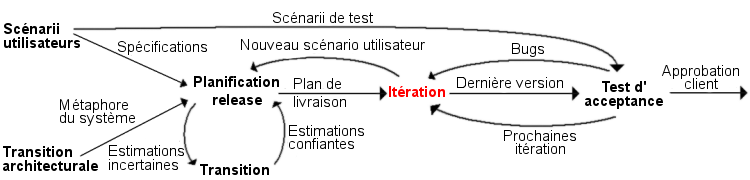
\includegraphics[width=15cm]{images/xp.png}
\caption{Cycle de l'Exreme Programing.}
\label{XP}
\end{figure}

Pour résumé, cette méthode nous ammène à réaliser la boucle suivante:
\begin{itemize}
\item Analyse du besoin.
\item Expression des spécifications
\item Réalisation technique
\item Test de la réalisation
\item Revue logicielle (validations qui permettront de faire évoluer le produit)
\end{itemize}\medskip

\section{Le cycle en V}
Le modèle du cycle en V est un modèle conceptuel de gestion de projet imaginé suite au problème de réactivité du modèle en cascade. Il permet, en cas d'anomalie, de limiter un retour aux étapes précédentes. Les phases \figref{cyclev} de la partie montante doivent renvoyer de l'information sur les phases en vis-à-vis lorsque des défauts sont détectés, afin d'améliorer le logiciel.

Le cycle en V est devenu un standard de l'Industrie logicielle depuis les années 1980 et depuis l'apparition de l'Ingénierie des Systèmes est devenu un standard conceptuel dans tous les domaines de l'Industrie. Le monde du logiciel ayant de fait pris un peu d'avance en termes de maturité, on trouvera dans la bibliographie courante souvent des références au monde du logiciel qui pourront s'appliquer au système.
\begin{figure}
\center
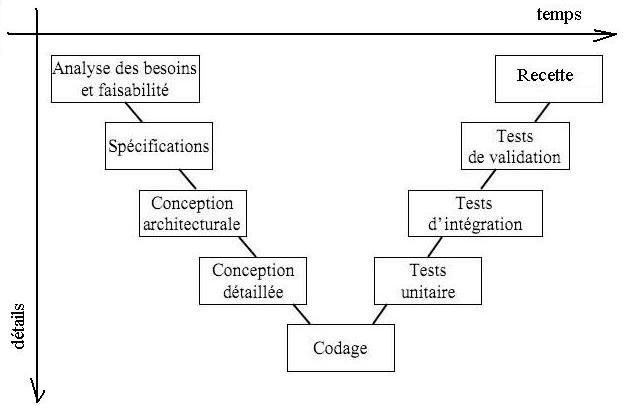
\includegraphics[width=12cm]{images/cyclev.png}
\caption{Les phases à travers le temps et le niveau de détails.}
\label{cyclev}
\end{figure}

Les étapes qui constitue cette méthode sont les suivantes :
\begin{itemize}
    \item Analyse des besoins et faisabilité
    \item Spécification logicielle
    \item Conception architecturale
    \item Conception détaillée
    \item Codage
    \item Test unitaire
    \item Test d'intégration
    \item Test de validation (Recette Usine, Validation Usine - VAU)
    \item Recette (Vérification d'Aptitude au Bon Fonctionnement - VABF)
\end{itemize}\medskip
 
On voit bien que dans notre cas, avec des besoins indefini, il est impensable d'appliquée une telle méthodologie sans engendrer le rique que le logiciel finial ne marche pas ou ne reponde pas aux attentes du client.

\section{Les avantages et inconvenients}
Les avantage de cette méthode, dans cette situation, serrons:
\begin{itemize}
    \item Enrichir le produit à chaque itération du cycle. Ci le logiciel marche le client peut visualiser immediatement les besoins qui etait superficiel, dont il n'avait pas réelement besoin, et au contraire découvrir de nouveau besoins réelement utile.
    \item Rediriger rapidement la conduite du projet. Si le client souhaite rediriger son projet, ceci peut etre fait dans les meilleur delai (changement d'objectifs ou de priorités)
    \item ... a completer.
\end{itemize}\medskip
 
Cette méthode implique tout de même un certain nombre d'inconvenient tel que:
\begin{itemize}
    \item Le client doit ètre disponible afin de faire avancer le projet. Chaque validation est vue avec le client et c'est celui-ci qui donne les nouveau besoins. Ce qui implique que ci celui-ci n'est pas disponible, le projet peut vite etre bloqué. 
    \item Le projet peut vite dériver. Ce type de méthode requiert des personnes compétente aussi bien au niveau Maitre d'ouvreage qu'au niveau maitre d'oeuvre. Il est facile de s'égarer c'est pourquoi une organisation et une rigeure doivent etre entretenue tout au long du projet.
    \item ... a completer.
\end{itemize}\medskip







    
